\documentclass{article}
\usepackage[frenchb]{babel}
\usepackage{amsfonts}
\usepackage{amsmath}
\usepackage[T1]{fontenc}
\usepackage[utf8]{inputenc}
\usepackage{amsthm}
\usepackage{graphicx}
\usepackage{tikz-cd}

\title{Bootstrap}
\author{ Cl\'ement Dell'Aiera, Guillaume Rateau}
\date{}

\theoremstyle{definition}
\newtheorem{definition}{Definition}
\newtheorem{thm}{Théorème}
\newtheorem{ex}{Exercice}
\newtheorem{lem}{Lemme}
\newtheorem{dem}{Preuve}
\newtheorem{prop}{Proposition}
\newtheorem{cor}{Corollaire}

\newcommand{\Z}{\mathbb Z}
\newcommand{\Q}{\mathbb Q}
\newcommand{\R}{\mathbb R}
\newcommand{\C}{\mathbb C}
\newcommand{\Hil}{\mathcal H}
\newcommand{\Mn}{\mathcal M _n (\mathbb C)}
\newcommand{\K}{\mathbb K}
\newcommand{\B}{\mathbb B}
\newcommand{\Cat}{\mathbb B / \mathbb K}

\begin{document}
\maketitle

\begin{abstract}

\end{abstract}


\newpage
\tableofcontents

\newpage

\setlength{\parindent}{0cm}
\section{Bootstrap et valeurs extrêmes}

\subsection{Théorèmes des valeurs extrêmes}


\begin{thm}
Si , pour une fonction de répartition $F$, il existe des suites réelles $a_n>0$ et $b_n$ telles que, en tout point de continuité de $F$ :
\[\lim_{n\infty} F^n(a_n x + b_n)=G_\gamma(x),\]
\noindent la loi limite $G$ est de la forme :
\[G_\gamma (x) = \exp(-(1+\gamma x )^{-\frac{1}{\gamma}}) \quad \text{pour} \ 1+\gamma x >0\]
\end{thm}

Le paramètre $\gamma$ donne de l'information sur la queue de la distribution : c'est un paramètre d'intérêt servant à prédire les évenements rares. Toutefois, les méthodes de Bootstrap naives ne fonctionnent plus dans le cas des valeurs extrêmes, à cause d'un potentiel biais.\\

\section{Estimation de la vitesse de convergence par régression}

Dans toute cette partie, l'échantillon considéré est stationnaire et est foretement mélangeant : \[\alpha(k)=\sup |P(A\cup B)-P(A)P(B)|\rightarrow 0 \quad \text{quand}\quad k\rightarrow\infty.\] 

On se donne un échantillon $X_1,..,X_n,..$ et une statistique d'intérêt $T_n$. Soit $Y_i$ le sous-échantillon $(X_i,X_{i+1}...,X_{i+b_n-1})$ pour $i\in[|1;q|]$ et $q=n-b_n+1$. Soit $T_{b_n,i}$ la statistique obtenue à partir de l'échantillon $Y_i$ avec le taux d'échantillonage $b_n$. On définit :
\[K_{b_n}(x|X^n,\tau)=\frac{1}{q}\sum_{i=1}^q  1_{\{\tau_n T_{b_n,i}\leq x\}}.\]

\begin{thm} \label{Reg} On suppose que : $||K_{b_n}(.|X^n,\tau)-K(.|P)||_\infty = o_P(1)$.\\
Si $K$ est continue et atteint ses bornes sur un compact, sur lequel elle est strictement croissante, alors, lorsque $n$ tend vers l'infini :
\[\tau_{b_n} K^{-1}_{b_n}(t|X^n)=K^{-1}(x,P)+ o_P(1)\]
\end{thm}

On se place dans les hypothèse \[\lim_{n\rightarrow +\infty} b_n=+\infty \quad \text{et}\quad\lim_{n\rightarrow +\infty}\frac{b_n}{n}=0.\]

Supposons que $\tau_n=n^{-\gamma}$. En passant au $\log$ dans la conclusion du théorème précédent, on obtient :
\[\log |K^{-1}_{b_n}(x|X^n,\tau)|=\log |K^{-1}(x,P)| + \gamma \log b_n +o_P(1).\]

En faisant alors varier les taux de sous-échantillonage $b_{n,i}$, on peut alors estimer $\gamma$ par moindres carrés ordinaires :

\[\hat\gamma=\frac{\sum_{i=1}^I(y_i-\overline y)(\log b_{i,n}-\overline\log)}{\sum_{i=1}^I(\log b_{i,n}-\overline\log)^2},\]
où $y_i=\log |K^{-1}_{b_{n,i}}(t|X^n)|$.\\

Une deuxième méthode est inspirée par la remarque suivante : il  suffit d'observer des différences de quantiles. En effet, si l'on prend l'équation du théorème \ref{reg} pour deux quantiles d'ordre $0<t_1<t_2$, et que l'on soutrait l'une à l'autre, après avoir passé au $\log$, on obtient :
\[\log|K^{-1}_{b_{n}}(t_1|X^n)-K^{-1}_{b_{n}}(t_2|X^n)| =\log|K^{-1}(t_1|P)-K^{-1}(t_2|P)|  + \gamma \log b_n +o_P(1).\]

Avec plusieurs quantiles d'ordre $0<t_1<....< t_J<1$, on obtient un système :
\[y_{ij}= \log|K^{-1}_{b_{n,i}}(t_j|X^n)|=a_j+\gamma \log b_{n,i}+u_{ij}, \]
où $a_j=\log|K^{-1}(t_j|P)| $ et $u_{ij}=o_P(1)$.\\

 Un estimateur de type ANOVA est 
\[\gamma_{IJ}=\frac{\sum_{i=1}^I(y_{i,.}-\overline y)(\log b_{i,n}-\overline\log)}{\sum_{i=1}^I(\log b_{i,n}-\overline\log)^2},\]

\begin{thm}
Soit $X$ une suite stationnaire et fortement mélangeante, dont la statistique d'intérêt $\tau_n T_n$ possède une distribution asymptotique, lorsque $\tau_n = n^{-\gamma}$, $\gamma>0$ inconnu. On suppose de plus que $K$ est strictement croissante sur un intervalle borné et continue. On choisit des point $t_j$ dans $(0,1)$ et différents taux de sous-échnatilonage $n^{\beta_i}$, $1>\beta_1>...>\beta_I>0$. Alors :
\[\gamma _{IJ}=\gamma +o_P((\log n )^{-1})\]
\end{thm}

\subsection{Applications à la théorie des valeux extrêmes. Simulations.}

\begin{figure}[!h]\centering
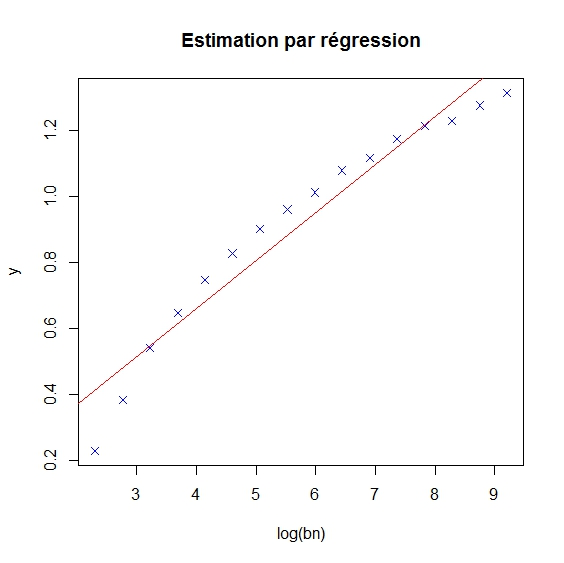
\includegraphics[scale=0.4]{RegGauss.jpeg}
\label{RegGauss}
\caption{Régression de $\log b_n$.}
\end{figure}


\bibliographystyle{plain}
\bibliography{biblio} 
\nocite{*}
\end{document}

























